% Fig. 3: shared controller structure (single column): sensing -> two command sources (learned layer | classical
% controller with its phase estimate) -> the gate selects one -> reflex and muscle layers -> actuators -> FlapSim.
% The pulse switch of the classical controller (off/on during manoeuvres) is drawn as a switch symbol.
% Build:  cd figures/tikz && pdflatex controller_diagram.tex   (needs flapsim_render.jpg in the same folder)
\documentclass[border=1pt]{standalone}
\pdfsuppressptexinfo=-1  % do not copy the info dictionaries (author names) of included PDFs
\pdfinfo{/Author () /Title ()}
\usepackage{newtxtext,newtxmath}
\usepackage{tikz}
\usetikzlibrary{arrows.meta,calc,positioning}
\definecolor{snn}{HTML}{1764D6}
\definecolor{snnedge}{HTML}{0B3D8C}
\definecolor{snnfill}{HTML}{EAF2FD}
\definecolor{snnlight}{HTML}{86B6EF}
\definecolor{cls}{HTML}{4A4844}
\definecolor{clsfill}{HTML}{EEEDE8}
\definecolor{ink2}{HTML}{52514E}
\definecolor{muted}{HTML}{898781}
\definecolor{grid}{HTML}{D9D7D0}
\definecolor{ok}{HTML}{1E8E3E}
\begin{document}
\begin{tikzpicture}[
    >={Stealth[length=5pt,width=4pt]},
    tiny/.style={font=\fontsize{7.2pt}{8.2pt}\selectfont, text=ink2, inner sep=1pt},
    lbl/.style={font=\fontsize{7.4pt}{8.4pt}\selectfont, text=black},
    box/.style={lbl, draw=ink2, line width=1.0pt, rounded corners=3pt, fill=white, align=center,
                inner xsep=3pt, inner ysep=2.5pt, minimum height=7.4mm},
    learn/.style={box, draw=snnedge, fill=snnfill},
    classic/.style={box, draw=cls, fill=clsfill},
    flow/.style={->, line width=1.1pt, draw=ink2},
  ]
  % ---------------- plant ----------------
  \node[inner sep=0] (sim) at (0.70,-2.45) {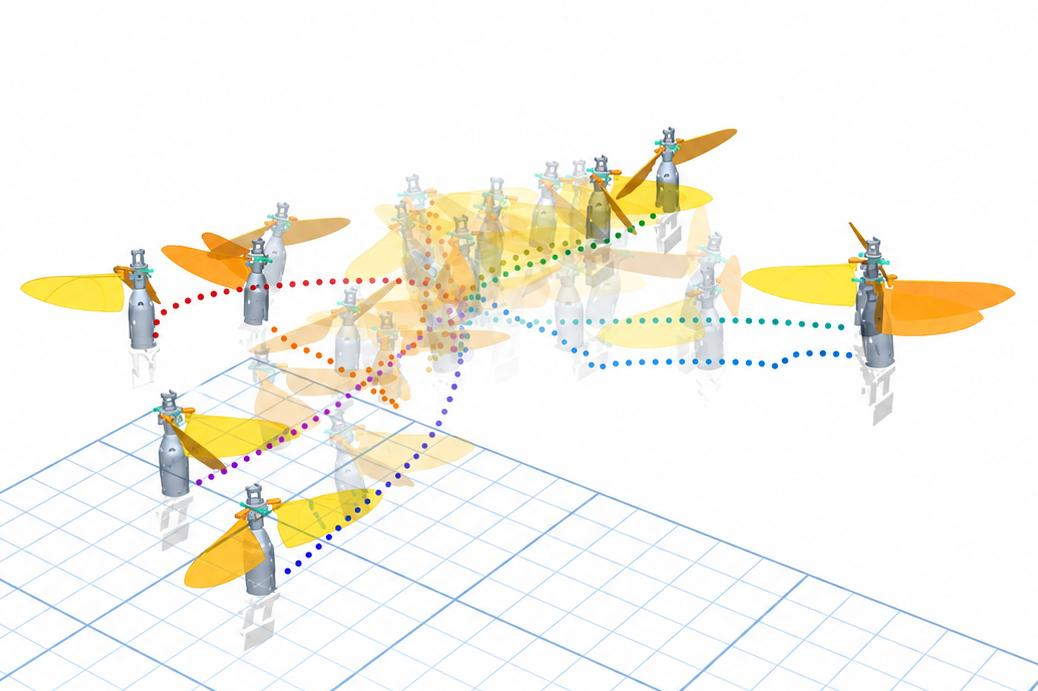
\includegraphics[width=1.3cm]{flapsim_render.jpg}};
  \node[font=\fontsize{7.6pt}{8.6pt}\selectfont\bfseries, below=.6mm of sim] (simlab) {FlapSim};

  % ---------------- sensing ----------------
  \node[box, minimum width=6.55cm, minimum height=6mm] (sens) at (5.515,0) {\textbf{Sensors:} IMU (attitude, rate, acceleration), range};

  % ---------------- command sources ----------------
  \node[learn, minimum width=3.1cm, text width=2.9cm] (cmd) at (3.79,-1.40)
    {\textbf{\color{snnedge}Learned command layer}\\ SNN (Fig.~1) or MLP + PPO\\ {\color{ink2}no phase input}};
  \node[classic, minimum width=3.1cm, text width=2.9cm, minimum height=1.39cm] (cls) at (7.24,-1.40)
    {\textbf{Classical controller}\\ set-point schedule\\ + pulse law\\ {\color{ink2}(PLL phase estimate)}};

  % ---------------- gate ----------------
  \node[box, minimum width=6.55cm, text width=6.3cm] (gate) at (5.515,-3.32)
    {\textbf{Gate:} learned layer in charge during a manoeuvre\\ and for 1\,s after it; classical controller otherwise};

  % ---------------- lower layers ----------------
  \node[box, minimum width=3.1cm] (reflex) at (3.79,-4.40) {\textbf{Reflex layer}\\ PID: set-points $\to$ gimbal};
  \node[box, minimum width=3.1cm] (muscle) at (7.24,-4.40) {\textbf{Muscle layer}\\ 6\,ms max.-speed pulse};

  % ---------------- actuators ----------------
  \node[box, minimum width=6.55cm, minimum height=6mm] (act) at (5.515,-5.38)
    {\textbf{Actuators:} gimbal $\alpha,\beta$ ($\pm0.3$\,rad), motor speed $\omega$};

  % ---------------- flows (no labels on lines) ----------------
  % plant -> sensors
  \draw[flow, rounded corners=3pt] (sim.north) ++(0,.05) |- (sens.west);
  % sensors -> command sources
  \draw[flow] (cmd.north |- sens.south) -- (cmd.north);
  \draw[flow] (cls.north |- sens.south) -- (cls.north);
  % command sources -> gate; the classical pulse law passes a manoeuvre switch (open = off)
  \draw[flow] (cmd.south) -- (cmd.south |- gate.north);
  \coordinate (swa) at ($(cls.south)+(0,-.14)$);
  \coordinate (swb) at ($(cls.south)+(0,-.42)$);
  \draw[cls, line width=1.1pt] (cls.south) -- (swa);
  \fill[cls] (swa) circle (.05);
  \fill[cls] (swb) circle (.05);
  \draw[cls, line width=1.1pt, line cap=round] (swa) -- ++(.26,-.21);
  \draw[flow] (swb) -- (cls.south |- gate.north);
  \node[tiny, anchor=east, align=right] at ($(swa)!.5!(swb)+(-.16,0)$) {pulse law during manoeuvres:\\[-1pt]off (open) or on};

  % gate -> lower layers -> actuators
  \draw[flow] (reflex.north |- gate.south) -- (reflex.north);
  \draw[flow] (muscle.north |- gate.south) -- (muscle.north);
  \draw[flow] (reflex.south) -- (reflex.south |- act.north);
  \draw[flow] (muscle.south) -- (muscle.south |- act.north);
  % actuators -> plant
  \draw[flow, rounded corners=3pt] (act.west) -| (simlab.south);
\end{tikzpicture}
\end{document}
